\documentclass[12pt]{extarticle}
\usepackage{geometry}
\geometry{
a4paper,
total={170mm,257mm},
left=20mm,
top=20mm,
headheight=12pt
}

\usepackage[parfill]{parskip} % Activate to begin paragraphs with an empty line rather than an indent
\usepackage{graphicx} % Use pdf, png, jpg, or eps§ with pdflatex; use eps in DVI mode
% TeX will automatically convert eps --> pdf in pdflatex		

\usepackage{amssymb,amsmath,amsthm}
\usepackage{commath}
\usepackage{longtable}
\usepackage[hyphens]{url}
\usepackage[dvipsnames]{xcolor}
\usepackage[unicode=true,colorlinks=true,urlcolor=CadetBlue,citecolor=black,linkcolor=black]{hyperref}
\PassOptionsToPackage{hyphens}{url} % url is loaded by hyperref
\usepackage{authblk}
\usepackage{subcaption}
\captionsetup[subfigure]{labelformat=empty}
\usepackage[font=small,labelfont=bf]{caption}

%SetFonts
% newtxtext+newtxmath
\usepackage{newtxtext} %loads helv for ss, txtt for tt
\usepackage{amsmath}
\usepackage[bigdelims]{newtxmath}
\usepackage[T1]{fontenc}
\usepackage{textcomp}
%SetFonts

% less space before sections 
% \@startsection {NAME}{LEVEL}{INDENT}{BEFORESKIP}{AFTERSKIP}{STYLE} 
%            optional * [ALTHEADING]{HEADING} 
\makeatletter
 \renewcommand\section{\@startsection {section}{1}{\z@}%
     {-2.5ex \@plus -1ex \@minus -.2ex}%
     {1.3ex \@plus.2ex}%
    {\Large\bfseries}}
    
% Species names
%% Meta-Command for defining new species macros
\usepackage{xspace}

\newcommand{\species}[3]{%
  \newcommand{#1}{\gdef#1{\textit{#3}\xspace}\textit{#2}\xspace}}
  
\species{\yeast}{Saccharomyces cerevisiae}{S.~cerevisiae}
\species{\calbicans}{Candida albicans}{C.~albicans}
\species{\cneoformans}{Cryptococcus neoformans}{C.~neoformans}

% Yoav & Lee commands
\newcommand*{\tr}{^\intercal}
\let\vec\mathbf
\newcommand{\matrx}[1]{{\left[ \stackrel{}{#1}\right]}}
\newcommand{\diag}[1]{\mbox{diag}\matrx{#1}}
\newcommand{\goesto}{\rightarrow}
\newcommand{\dspfrac}[2]{\frac{\displaystyle #1}{\displaystyle #2} }
\newtheorem{theorem}{Theorem}
\newtheorem{corollary}{Corollary}
\newtheorem{lemma}{Lemma}
\newtheorem{remark}{Remark}
\newtheorem{result}{Result}
\renewcommand\qedsymbol{} % no square at end of proof
\newcommand{\cl}{\mathbf{L}}
\newcommand{\cj}{\mathbf{J}}
\newcommand{\ci}{I}

% NatBib
\usepackage[round,colon,authoryear]{natbib}

% Title page
% Chromosomal duplication is a transient evolutionary solution to stress
\title{Clonal interference between aneuploidy and mutation}

% Authors
\renewcommand\Affilfont{\small}

\author[1]{Ilia Kohanovski}
%\author[b,c]{Avihu H. Yona}
%\author[d]{Orna Dahan}
%\author[d]{Yitzhak Pilpel}
\author[1,2,*]{Yoav Ram}

\affil[1]{School of Computer Sciences, IDC Herzliya, Herzliya, Israel}
\affil[2]{School of Zoology, Faculty of Life Sciences, Tel Aviv University, Tel Aviv, Israel}
%\affil[b]{Department of Physics, Massachusetts Institute of Technology, Cambridge, MA 02139, USA}{
%\affil[b]{Department of Biological Engineering, Massachusetts Institute of Technology, Cambridge, MA 02139, USA}
%\affil[d]{Department of Molecular Genetics, Weizmann Institute of Science, Rehovot 76100, Israel}
\affil[*]{Corresponding author: yoav@yoavram.com}

% Document
\begin{document}
\maketitle

% Abstract
\begin{abstract}
Aneuploidy is common in eukaryotes, often leading to decreased cell growth and fitness. However, evidence from yeast and fungi, as well as tumour cells, suggests that aneuploidy can be beneficial under stressful conditions and  lead to elevated growth rates and to adaptation. Thus, it is crucial to develop a quantitative theory for the role of aneuploidy in adaptive evolution. Here, we analyse results from experiments in which \yeast adapted to heat stress. The experimental population first acquired chromosome duplications, only to later revert back to a euploid state. We use several evolutionary models within a approximate Bayesian computation framework to show that clonal interference between chromosome duplications and beneficial mutations explains the experimental results. Our results suggest that aneuploidy can both accelerate and deccelerate adaptation in a non-intuitive manner, creating an evolutionary conflict between the individual and the population and further complicating the process of adaptation in cell populations.
\end{abstract}

\pagebreak
% Introduction
\section*{Introduction}

\paragraph*{Aneuploidy is common in eukaryotes.}
Aneuploidy is an imbalance in the number of chromosomes in the cell: an incorrect karyotype.
Recent evidence suggests aneuploidy is very common in eukaryotes, e.g. animals~\citep{Santaguida2015review, Naylor2016, Bakhoum2017}, and fungi~\citep{Pavelka2010, Zhu2016, Robbins2017, Todd2017}.
Aneuploidy has been implicated in cancer formation and progression~\citep{Boveri2008, Schvartzman2010}: 
90\% of solid tumours and 50\% of blood cancers are aneuploid~\citep{Santaguida2015review}.
Aneuploidy is also linked to the emergence of drug resistance~\citep{Selmecki2009} and virulence~\citep{Moller2018} in fungal pathogens, which are under-studied~\citep{Rodrigues2018} despite infecting close to a billion people per year, causing serious infections and significant morbidity in >150 million people per year and killing >1.5 million people per year~\citep{Selmecki2009, Rodrigues2018}.
In addition, aneuploidy is common in protozoan pathogens of the Leishmania genus, a major global health concern~\citep{Mannaert2012}.

\paragraph*{Aneuploidy is generally deleterious.}
The molecular and genetic mechanisms involved in aneuploidy have been explored in the past decade~\citep{Musacchio2007, Sheltzer2011, Chen2012b, Rancati2013, Gerstein2015, Shor2015}.
Experiments with human and mouse embryos found that aneuploidy is usually lethal;
it is also associated with developmental defects and lethality in other multicellular organisms~\citep{Sheltzer2011}. For example, aneuploid mouse embryonic cells grow slower than euploid cells~\citep{Williams2008}.
Similarly, in unicellular eukaryotes growing in benign conditions, aneuploidy usually leads to slower growth and decreased overall fitness~\citep{Niwa2006, Torres2007, Pavelka2010, Sheltzer2011, Kasuga2016}, in part due to proteotoxic stress caused by increased expression in aneuploid cells~\citep{Pavelka2010, Santaguida2015, Zhu2018} and hypo-osmotic-like stress~\citep{Tsai2019}.

\paragraph*{Aneuploidy can lead to adaptation.}
However, aneuploidy can be beneficial under stressful conditions due to the wide range of phenotypes it can produce, some of which are advantageous~\citep{Pavelka2010}.
Thus, aneuploidy can lead to rapid adaptation in unicellular eukaryotes~\citep{Gerstein2015,Torres2010, Hong2014, Rancati2008}, as well as to rapid growth of somatic tumour cells~\citep{Schvartzman2010, Sheltzer2017}.
For example, aneuploidy in \yeast facilitates adaptation to a variety of stressful conditions like heat and pH~\citep{Yona2012}, copper~\citep{Covo2014, Gerstein2015}, salt~\citep{Dhar2011}, and nutrient limitation~\citep{Dunham2002, Gresham2008}.
Importantly, aneuploidy can also lead to drug resistance in pathogenic fungi such as \calbicans~\citep{Selmecki2008, Selmecki2010, Gerstein2018} and \cneoformans~\citep{Sionov2010}, which cause candidiasis and meningoencephalitis, respectively.

\paragraph*{Transient adaptive solution.} 
Aneuploidy differs from mutation due to its distinct properties. 
Chromosome duplication usually occurs more often than mutation and on average produces larger fitness effects.
Yet, because it affects many genes on a whole chromosome or a chromosome fragment, aneuploidy also carries fitness costs.
Thus, aneuploidy can be a \emph{transient adaptive solution}: it can rapidly occur and fix in the population under stressful conditions, and can be rapidly lost when the cost outweighs the benefit -- when stress is removed or after beneficial mutations occur.
Experimental evidence of such a transient role of aneuploidy was demonstrated by \citet{Yona2012}, who evolved populations of \yeast under strong heat or pH stress.
In these experiments, the populations quickly adapted to the stress, and this adaptation was determined to be due to chromosome duplications.
Later on, the populations reverted back to an euploid state, while remaining adapted to the stress and accumulating multiple mutations.
However, under gradual heat stress, aneuploidy was not observed.
\citet{Yona2012} concluded that aneuploidy serves as a transient adaptive solution, or a ``quick fix'', which is expected to facilitate adaptation. 

\paragraph*{The present study.}
Here, we develop a series of computational evolutionary models that include the effects of natural selection, genetic drift, aneuploidy and mutation to examine the role of aneuploidy in adaptation.
These models follow a population of cells characterised by both their ploidy and their genotype.
We fit these models to the empirical results of \citet{Yona2012} using approximate Bayesian computation.
These model fits allow us to infer model parameters, including selection coefficients and transition rates, and to perform model selection between different models, thereby testing different hypotheses about the evolutionary process.
We find that % TODO CHECK!
the aneuploidy rate is several orders of magnitude higher than the mutation rate; that a simple model of clonal interference is not enough to explain the transience of aneuploidy; and that aneuploidy rescues the population, albeit at the price of delaying further adaptation.

\pagebreak
% Models and Methods
\section*{Models and Methods}

\paragraph*{Evolutionary Models.} To examine the role of aneuploidy in adaptation, two models were developed - \emph{single-mutant model} and \emph{multiple-locus model}. 
Both are based on the Wright-Fisher model~\citep{Tenaillon1999} and include the effects of natural selection, genetic drift, aneuploidy, and mutation. Only beneficial mutations assumed, 
thus neglecting the effects of deleterious and neutral mutations. The \emph{single-mutant model} allows for a single mutation (on specific locus or target loci), while the 
\emph{multiple-locus model} allows for multiple mutations. Both models allow for a single aneuploid karyotype (e.g. chromosome III duplication). (\autoref{fig:models})

\begin{figure}[b!]
  \centering
  \begin{subfigure}[t]{0.5\textwidth}
      \centering
      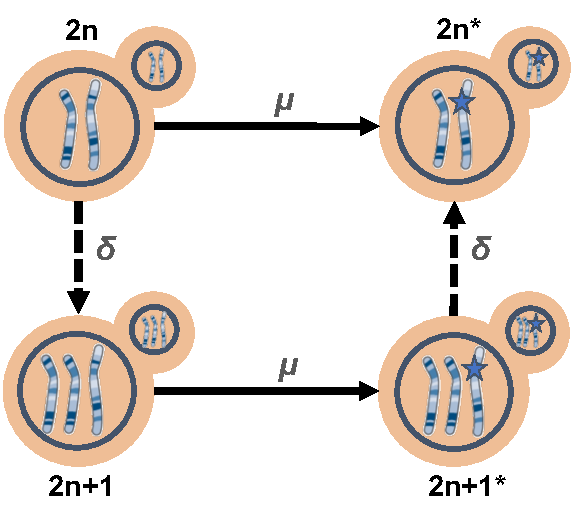
\includegraphics[height=1.8in]{../figures/Fig1-A.pdf}
      \caption{
        \textbf{A. Single-mutant}
        }
      \label{fig:model1}
  \end{subfigure}%
  ~ 
  \begin{subfigure}[t]{0.5\textwidth}
      \centering
      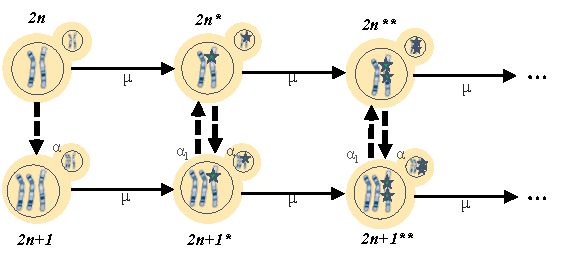
\includegraphics[height=1.8in]{../figures/Fig1-B.pdf}
      \caption{
        \textbf{B. Multiple-locus}
      }
      \label{fig:model2}
  \end{subfigure}
  \caption{
    \textbf{Model Schemes.} (A) The population with four possible genotypes and four possible transitions from one genotype to another with the transition rates $\mu$, $\alpha$, 
    $\alpha_l$, $k\mu$. \emph{2n}: euploid wildtype – the initial genotype; \emph{2n*}: euploid mutant, standard karyotype with one specific beneficial mutation; 
    \emph{2n+1}: aneuploid wildtype, with an extra chromosome, e.g. following chromosome duplication; \emph{2n+1*}: 
    aneuploid mutant, with both the beneficial mutation and the extra chromosome. Overall there are two possible paths to reach \emph{2n*} from \emph{2n}.
    (B) Each genotype can have zero or more beneficial mutations and zero or one extra chromosomes. $\mu$, mutation rate; $\alpha$, aneuploidy gain rate; $\alpha_l$, aneuploidy loss rate
  }
  \label{fig:models}
\end{figure}

\paragraph*{Single-mutant model.} It contains four predefined genotypes whose frequencies change during generations. \emph{2n}: euploid wildtype - the initial genotype; 
\emph{2n*}: euploid mutant, standard karyotype with one specific beneficial mutation; \emph{2n+1}: aneuploid wildtype, with an extra chromosome, e.g. following chromosome duplication; 
\emph{2n+1*}: aneuploid mutant, with both the beneficial mutation and the extra chromosome. 

The parameters of the model are: 
$N$, the population size, which is constant in all generations; $\mu$, the mutation rate - the transition rate from \emph{2n} to \emph{2n*}, i.e. the frequency at which cells with genotype \emph{2n*}
are created from cells with genotype \emph{2n}; $\alpha$, the aneuploidy gain rate - the transition rate from \emph{2n} to \emph{2n+1}; 
$\alpha_l$, the aneuploidy loss rate - the transition rate from \emph{2n+1*} to \emph{2n*}; $k$, the coefficient, such that $k\cdot\mu$ is the transition rate from \emph{2n+1} to \emph{2n+1*}, 
where on default $k$ is equals to $33/32$ (euploid \emph{2n} genotyped \emph{S. cerevisiae} contains 32 chromosomes, therefore, assuming each chromosome have equal probability to have the specific 
beneficial mutation in, aneuploid \emph{2n+1} genotype should have 33/32 times the mutation rate); $s$, the mutation selection coefficient; $s_b$, fitness benefit of aneuploidy; 
$c$, fitness cost of aneuploidy, where $0<c<1$. The relative finesses of genotypes are:
\begin{equation} \label{eq:single-w} \begin{aligned}
w_{2n} & = 1 \\
w_{2n+1} & = 1-c+s_b \\
w_{2n+1*} & = (1+s)(1-c)+s_b \\
w_{2n*} & = (1+s) \;
\end{aligned}
\end{equation}

\pagebreak

The model follows Wright-Fisher \citep{Tenaillon1999} steps. The first generation is initialized with $N$ cells of the genotype \emph{2n}. At each generation, the frequency $f_g$ of 
each genotype $g$ is updated:
\begin{enumerate}
  \item Selection step: 
    \begin{equation} \label{eq:single-selection} 
      f_g\gets{\dfrac{f_g w_g}{\sum_{j}f_j w_j}}
      %  j\in\{2n, 2n+1, 2n+1*, 2n*\} 
    \end{equation}
  \item Mutation gain and aneuploidy gain/loss step:
    \begin{equation} \label{eq:single-mutation} \begin{aligned}
      f_{2n} & \gets{f_{2n} - \alpha f_{2n} - \mu f_{2n}}  \\
      f_{2n+1} & \gets{f_{2n+1} - k\mu f_{2n+1} + \alpha f_{2n}}  \\
      f_{2n+1*} & \gets{f_{2n+1*} - \alpha_l f_{2n+1*} + k\mu f_{2n+1}}  \\
      f_{2n*} & \gets{\mu f_{2n} + \alpha_l f_{2n+1}}  \;
    \end{aligned}
    \end{equation}
  \item Random drift step: draw the frequencies of all genotypes from a multinomial distribution
    \begin{equation} \label{eq:single-mutation} 
      f \sim Mult(N, (f_{2n},f_{2n+1},f_{2n+1*},f_{2n*}))
    \end{equation}
\end{enumerate}



\paragraph*{Multiple-locus model.} It expands the \emph{single-mutant model} by allowing for any number of beneficial mutations. For each mutation $i$, selection coefficient $s_i$ is independently drawn from an exponential distribution with expected value $s$. The parameters of the model are $\mu$, the mutation rate; $\alpha$, the aneuploidy gain rate; $\alpha_l$, the aneuploidy loss rate; $s$, the parameter of the exponential distribution; $s_b$, fitness benefit of aneuploidy; $c$, fitness cost of aneuploidy, where $0<c<1$. In this model, the population may include any number of genotypes that contain zero or more mutations and zero or one extra chromosomes. The fitness $w_g$ of genotype $g$ is: 

\begin{equation} 
w_g= 
\begin{cases}
   1, & \text{wildtype} \\
	1-c+s_b, & \text{aneuploid wildtype} \\
	\prod_{\text{i is mutation in g}}{(1+s_i)}, & \text{euploid mutant} \\ 
	s_b+(1-c)\prod_{\text{i is mutation in g}}{(1+s_i)}, & \text{aneuploid mutant}
\end{cases}
\end{equation}

Therefore, aneuploidy loss would be favored by selection only if there are enough beneficial mutations or/and the mutation selection coefficients $s_i$ are large enough. The intuition is as follows: when the benefit of the accumulated beneficial mutations is small, then the benefit of aneuploidy has a large effect; when the benefit of the accumulated beneficial mutations benefit is large, then aneuploidy doesn’t add much, and its cost becomes significant.

Unlike the single-locus model, the population size for the multiple-locus model is not constant. Indeed, a serial-transfer protocol~\citep{Barrick2013} is simulated, where the population is repeatedly diluted by transfer to a fresh medium, starting a new growth cycle, similar to the original experiment. In the model the population initial size is $N$, then it is doubled every iteration till reaching $8\cdot{N}$, then it is diluted back to $N$.

Denote by $n_g$ be the number of cells of genotype $g$ in the population. At each generation, genotypes frequencies are changed by the following steps:
\begin{enumerate}
	\item Selection step: 
	\begin{equation} \label{eq:multiple-selection} 
		n_g\gets{n_g\cdot{w_g}}
	\end{equation}
	\item Random drift step:
	\begin{equation} \label{eq:multiple-rand-drift} \begin{aligned}
			f \sim Mult(N', (\frac{n_1}{N'},\frac{n_2}{N'},...)) \text{ where } N'=n_1+n_2+... 
		\end{aligned}
	\end{equation}
	\item Normalization after N change (growth or dilution):
	\begin{equation} \label{eq:multiple-pop-size} 
		n_g\gets{f_g\cdot{N}}
	\end{equation}
\end{enumerate}



 
\pagebreak
% Results
\section*{Results}

\pagebreak
% Discussion
\section*{Discussion}

\paragraph*{Aneuploidy and mutation: \textit{same-same but different}.}
The published data indicate that, like mutation, aneuploidy can be both deleterious and beneficial~\citep{Pavelka2010, Sheltzer2011}.
Nevertheless, there are important and fundamental differences between adaptation by aneuploidy
and adaptation by beneficial mutations~\citep{Yona2015}, which make aneuploidy a unique mechanism for generating genetic
variation.
First, the aneuploidy rate (i.e. the frequency of mis-segregation events) is significantly higher than the
mutation rate~\citep{Santaguida2015review}.
Thus, everything else being equal, adaptation by aneuploidy will be faster and more frequent.
Second, fitness effects of aneuploidy are larger than those of the majority of mutations, on average, and are rarely
neutral~\citep{Pavelka2010, Yona2012, Sunshine2015}, allowing selection to quickly sort deleterious and beneficial genotypes.
Third, the number of different karyotypes is considerably smaller than the number of different genotypes, and different karyotypes are likely to have different phenotypes~\citep{Pavelka2010}.
Therefore, exploration of the phenotype space by aneuploidy requires smaller populations and a shorter time span.
Fourth, aneuploidy is a reversible state, as the rate of chromosome loss is high and the cost of aneuploidy is significant~\citep{Niwa2006}.
Indeed, aneuploidy often provides a transient solution: under short-term stress conditions, aneuploidy reverts (chromosome number returns to normal) when the stress subsides; under long-term stress conditions, aneuploidy reverts when refined solutions, generated by beneficial mutations, take over~\citep{Yona2012}.
Finally, aneuploidy results in increased genome instability, potentially increasing genetic variation by a positive feedback loop~\citep{Rancati2013, Bouchonville2009, Zhu2012}, while also increasing its own transience.

\paragraph*{Evolutionary theory of aneuploidy.}
The role of aneuploidy in adaptation has only recently been observed~\citep{Sionov2010, Yona2012, Gerstein2015}, and is largely missing from the literature on evolution and adaptation:
the introductory textbook \emph{Evolution} by~\citet{Bergstrom2012} does not mention the word aneuploidy, and the graduate-level book \emph{Mutation-Driven Evolution} by~\citet{Nei2013} only briefly mentions aneuploidy in the context of speciation, but not adaptation.
In recent reviews of the literature, aneuploidy is suggested to play an important role in fungal adaptation~\citep{Robbins2017, Todd2017} and cancer evolution~\citep{Santaguida2015review, Naylor2016, Sansregret2017}, yet these reviews cite no theoretical studies nor any quantitative models.
Indeed, evolutionary, ecological, and epidemiological studies mostly assume adaptation occurs via beneficial mutations, recombination, and sex.
Therefore, there is a critical need to develop an evolutionary theory of aneuploidy like the evolutionary theories of other mechanisms for generation of genetic variation, e.g. mutation~\citep{Lynch2010}, recombination~\citep{Hartfield2012}, and sex~\citep{Otto2009}.
An evolutionary theory of aneuploidy will be central to the interpretation of experimental and clinical observations and design of new hypotheses, experiments, and treatments~\citep{Carja2014}.
For example, despite the lack of theoretical models, aneuploidy has been invoked in a new strategy to combat pathogens and tumour cells by setting “evolutionary traps”~\citep{Gerstein2015,Chen2015}, in which a condition that predictably leads to emergence of aneuploidy is applied, followed by a condition that specifically selects against aneuploid cells.

\pagebreak
% Acknowledgements
{\small
\section*{Acknowledgements}
We thank Lilach Hadany, Judith Berman, David Gresham, and Martin Kupiec for discussions and comments.
This work was supported in part by 
the Israel Science Foundation 552/19 and Minerva
Stiftung Center for Lab Evolution (YR).
}

\bibliographystyle{agsm}
\bibliography{ms.bib}

\end{document}  